\section{Grundsätzliches zum Regelkreis}
\subsection{Definitionen \skript{9-24}}


\begin{description}[leftmargin=2.5cm]
 \item[System]	Eine Anordnung von Gebilden, welches von der Umwelt abgegrenzt ist, aber
								mit ihr über Inputs/Outputs in einer Beziehung stehen.\quad{\color{red} Skript S.19}
 \item[Prozess] Die Gesamtheit der zusammenwirkenden Vorgänge in einem System,
        		durch die Materie, Energie, Informationen umgeformt, transportiert und
        		gespeichert wird.\quad{\color{red} Skript S.19} \\
        		\begin{tabular}{lp{12cm}}
        		\textbf{ohne Ausgleich:} & Die Ausgangsgrösse ist für $t \rightarrow \infty$ nicht begrenzt \\
        		\textbf{mit Ausgleich:} & Die Ausgangsgrösse ist für $t \rightarrow \infty$ begrenzt. Ein Prozess wo sich selber ausgleicht wird oft mit einem $PT_1$-Glied modelliert.
        		\end{tabular}
 \item[Modell]	Ein Modell ist eine Abbildung eines Systems in ein anderes begriffliches oder
								gegenständliches System, dass den Prozess bezüglich ausgewählter Fragestellung
								hinreichend genau beschreibt.\quad{\color{red} Skript S.19}
 \item[SISO] Single Input - Single Output\quad{\color{red} Skript S.23}
 \item[MIMO] Multi Input - Multi Output\quad{\color{red} Skript S.23}
 \item[Steuerung]	Bei einer Steuerung wird der Energiestrom über mindestens einen Verstärker (Stelleinrichtung)
									beeinflusst, so dass die Prozessaufgabe erfüllt wird, wobei die Steuerinformation
									von Glied zu Glied läuft (Steuerkette) {\color{red} Skript S.18} \newline
									- ohne Rückkopplung \newline
									- kann bei \underline{stabiler} Strecke \underline{nicht instabil} werden \newline
									- open loop\\
	\begin{minipage}{8cm}
		 \item[Regelung] mit Rückkopplung (wirkt als Gegenkopplung) \\{\color{red} Skript S.18} \newline
		 				 - immer ein Vergleichsglied zwischen Führungsgrösse (Sollwert) und
		 				   Regelgrösse (Istwert) \newline
		 				 - kann auf veränderte Störgrössen reagieren \newline
		 				 - kann bei \underline{stabiler} Strecke \underline{instabil} werden. \newline
						 - closed loop
						 - gutes Führungsverhalten: Normalerweise will man, dass die Regelgrösse der Führungsgrösse entspricht. \newline
						 \textbf{Festwertregelung} r(t) ist konstant {\color{red} Skript S.14} \newline
						 \textbf{Folgeregelung} r(t) variiert mit der Zeit {\color{red} Skript S.14}\newline
	\end{minipage}
	\begin{minipage}{9cm}
		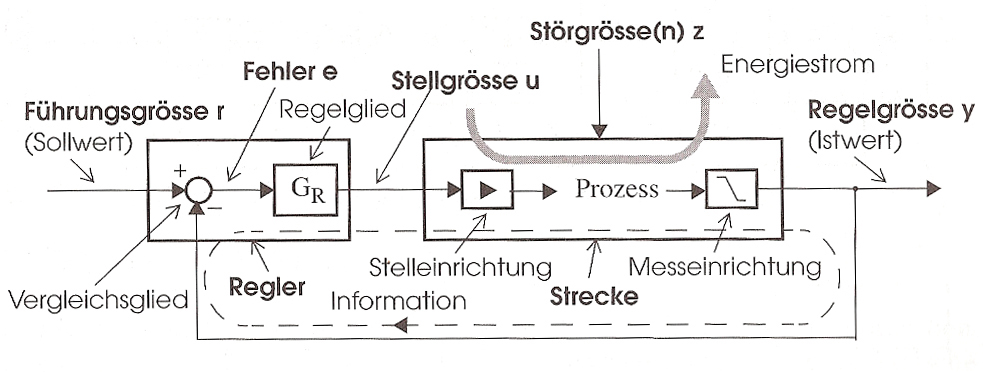
\includegraphics[width=\textwidth]{./bilder/Grundregelkreis_klein.jpg}
	\end{minipage}				
				
\end{description}

	\begin{tabular}{|p{2.7cm}|p{5.4cm}|l|}
    	\hline
    	{\bf Begriff deutsch}		&{\bf Begriff englisch}	&{\bf Ergänzende
    	Erklärung} \skript{13}\\
		\hline
		Regelung			& closed loop control ; control loop & Regelkreis\\
		\hline
		Regelstrecke		& plant controlled system	&Der aufgabengemäss zu beeinflussende
    	Teil des Systems\\
    	\hline
    	Regler				& controller			&Bestehent aus Vergleichsglied und Regelglied\\
    	\hline
    	Regeleinrichtung	& controlling means&\\
    	\hline
    	Reglesignalkreis	& control circuit&\\
    	\hline
    	Vergleichsglied		& comparing element	&Bildet den Fehler (Differenz)
    											e=r-y\\
    	\hline
    	Regelglied			&controller;
    						controlling element	&Berechnet aus dem Fehler die Stellgrösse u\\
    	\hline
    	Stelleinrichtung
    	Verstärker			&actuator;
					    	power amplifier;
    						servo amplifier		&Funktionseinheit, die den Energie- oder Massenstrom
    											lenkt\\
    	\hline
    	Messeinrichtung
    	Messumformer		&measuring unit;
    						transmitter&\\
    	\hline
    	Regelgrösse y		&controlled variable;
    						desiered value& auch c oder x (DIN)\\
    	\hline
    	Führungsgrösse r	&reference variable;
    						set value& w (DIN)\\
    	\hline
    	Störgrösse z Last	&disturbance variable;
    						load& auch d\\
    	\hline
    	Stellgrösse u		&manipulatetd (correcting)
    						variable& y (DIN)\\
    	\hline
    	Regeldifferenz e	&deviation ; error variable		& Fehler: $e=r-y \quad \quad x_d=w-x$ (DIN) \\
    	\hline
    	Rückkopplung		&feedback			&Rückführung\\
    	\hline

	\end{tabular}\\

		
	%\begin{sidewaystable}
	\subsection{Klassifizierung technischer Systeme}
		
		\begin{tabular}{|l|p{6.3cm}||l|p{6.3cm}|}
			
	        \hline
	        	
	        	einfach & 
	        	Bedeutung des \textbf{ersten} Begriffs & 
	        	schwierig & 	
	        	Bedeutung des \textbf{zweiten} Begriffs\\
	        \hline
	        	
	        	statisch &
	        	System ohne Gedächtnis.
	        	Wert am Ausgang hängt nur von gegenwärtigen
	        	Werten am Eingang ab.&
	        	\textcolor{blue}{\underline{dynamisch}} &
	        	System mit Gedächtnis.
	        	Wert am Ausgang hängt von gegenwärtigen
	        	und/oder vergangenen und/oder zukünftigen
	        	Werten am Eingang ab.\\
	        \hline
	        	
	        	\textcolor{blue}{\underline{linear}}	&
	        	Linearkombination am Eingang ruft
	        	entsprechende Linearkombination am
	        	Ausgang hervor.
	        	Nur Eingang x(t) muss linear sein,
	        	variable Faktoren f(t) nicht (z.B. sin(t))! &
	        	nichtlinear &
	        	Systeme die neue Frequenzanteile erzeugen.\\ %TODO Was ist damit gemeint: Ausnahmen: 2-, 3-Pt.Regler Simulation
	       	\hline
	        	
	        	\textcolor{blue}{\underline{zeitinvariant}} &
	        	Zeitliche Verschiebung des Eingangs ruft
	        	identische zeitliche Verschiebung am
	        	Ausgangs hervor. &
	        	zeitvariant	&
	        	Zeitinvarianz ist nicht erfüllt. \\
	        \hline
	        	
	        	\textcolor{blue}{\underline{Zeitkontinuierlich}} &
	        	Signal hat zu jedem Zeitpunkt einen Wert&
	        	zeitdiskret&
	        	\\
	        	$\dot{y}=\frac{ku-y}{T}$ &
	        	&
	        	$y_{k+1}=a y_k + b u_k$&
	        	\\
	        \hline
	        	
	        	\textcolor{blue}{\underline{wertkontinuierlich}}&
	        	Signal kann alle Werte eines Intervalles annehmen&
	        	wertdiskret&
	        	\\
	       	\hline
	        	
	        	\textcolor{blue}{\underline{kausal}}	&
	        	Wert am Ausgang hängt von gegenwärtigen 
	        	und/oder vergangenen Werten am Eingang ab.	&
	        	akausal&
	        	Wert am Ausgang hängt von zukünftigen
	        	und/oder gegenwärtigen und/oder vergangenen
	        	Werten am Eingang ab.\\
	       	\hline
	       
%TODO: Was ist damit gemeint 	
%	        	\textcolor{blue}{\underline{konzentrierte}} &
%	        	verteilte &
%	        	zB.	Stromleitung: &
%	        	\\
%	        	\textcolor{blue}{\underline{Parameter}} &
%	        	Parameter	&
%	        	ein R und ein C/ sehr viele RC-Glieder in Serie &
%	        	\\
%	        \hline
	        	
	        	\textcolor{blue}{\underline{deterministisch}}	&
	        	 Das Zeitverhalten lässt sich aufgrund seiner Gleichungen
	        	 ``reproduzieren"&
	        	stochastisch &		%vorhersehbar/zufällig
	        	\\
	        \hline
	        \hline
	        	reell&
	        	Reelles Eingangssignal bewirkt
	        	reelles Ausgangssignal.&
	        	
	        	invertierbar&
	        	Bei jedem Ausgangssignal kann eindeutig
	        	auf das entsprechende Eingangssignal
	        	geschlossen werden.\\
	        \hline
	        
	       \end{tabular}\\[1mm]
   				\textcolor{blue}{\underline{wird für Regler vorausgesetzt!}}
			
       % \end{sidewaystable}